\documentclass{article}
% set margins
\usepackage[left=1.5in, right=1in, top=1in, bottom=1in]{geometry}
% add spacing
\usepackage{setspace}
% use biblatex
\usepackage[style=numeric]{biblatex}
% add the bibliography
\addbibresource{bibliography.bib}
% remove dots in TOC
\usepackage[titles]{tocloft}
\renewcommand{\cftdot}{}

\usepackage{amssymb}
\usepackage{amsmath}

% unbold things
\usepackage{titlesec}
\titleformat*{\section} {\centering} % format
\titleformat*{\subsection}{\centering \normalfont}
\titleformat*{\subsubsection}{\normalfont}

\setcounter{tocdepth}{2}

% use images from the 'images' directory
\usepackage{graphicx}
\graphicspath{{images/}}

% place csv files in the thesis
\usepackage{csvsimple}
\usepackage{longtable}

% metadata
\title{Exploring Semantic Hierarchies to Improve Resolution Theorem Proving on Ontologies}
\author{Stanley C. Small}
\date{March 2019}

\begin{document}
\begin{titlepage}
	\makeatletter
		\begin{center}
   				\MakeUppercase{\@title} \par
  				\smallskip 
 				\vspace{.15in} by \par
 				\smallskip
  				\vspace{.15in} \@author \par
  				\vspace{1in}
 				A Thesis Submitted in Partial Fulfillment  \par
  				of the Requirements for a Degree with Honors \par
  				(Computer Science) \par
  				\vspace{.75in}
  				The Honors College \par
  				University of Maine \par
  				\@date \par
 				\vfill
   		\end{center}
	\makeatother
	\begin{flushleft}
		Advisory Committee: \\
		\hspace{.3in} Dr. Torsten Hahmann, Assistant Professor$^{1}$, Advisor \\
		\hspace{.3in} Dr. Mark Brewer, Professor of Political Science \\
		\hspace{.3in} Dr. Max Egenhofer, Professor$^{1}$ \\
		\hspace{.3in} Dr. Sepideh Ghanavati, Assistant Professor$^{1}$ \\
		\hspace{.3in} Dr. Roy Turner, Associate Professor$^{1}$ \\
		\hfill \break
		\hspace{.3in} $^{1}$School of Computing and Information Science
	\end{flushleft}
\end{titlepage}

\pagenumbering{gobble}
\newpage
\addcontentsline{toc}{section}{\MakeUppercase{Abstract}}
\setstretch{2}
\vspace*{.05in}
\section*{\MakeUppercase{Abstract}}
A resolution-theorem-prover (RTP) evaluates the validity (truthfulness) of conjectures against a set of axioms in a knowledge base. When given a conjecture, an RTP attempts to resolve the negated conjecture with axioms from the knowledge base until the prover finds a contradiction. If the RTP finds a contradiction between the axioms and a negated conjecture, it proves the conjecture. 

The order in which the axioms within the knowledge-base are evaluated significantly impacts the runtime of the program, as the search-space increases exponentially with the number of axioms. 

Ontologies, knowledge bases with semantic (and predominantly hierarchical) structures, describe objects and their relationships to other objects. For example, a 'Car' class might exist in a sample ontology with 'Vehicle' as a parent class and 'Bus' as a sibling class. Currently, any hierarchical structures within an ontology are not taken into account when evaluating the relevance of each axiom. At present, each predicate is automatically assigned a weight based on a heuristic measure (such as the number of terms or the frequency of predicates relevant to the conjecture) and axioms with higher weights are evaluated first. My research aims to intelligently select relevant axioms within a knowledge-base given a structured relationship between predicates. I will use the semantic hierarchy over predicates to assign weights to each predicate passed to a weighting function. The research aims to design heuristics based upon the semantics of the predicates, rather than solely the syntax of the statements. 

I plan to develop weighting functions based upon various parameters relevant to the ontological structure of predicates contained in the ontology, such as the size and depth of a hierarchy based upon the structure of the ontology. 

I will implement methods to calculate weights for each predicate and thus each axiom in attempts to select relevant axioms when proving a theorem. Then, I will conduct an experimental study to determine if my methods show any improvements over current reasoning methods.
	
\pagenumbering{roman} 
\setcounter{page}{3}
\newpage
\addcontentsline{toc}{section}{\MakeUppercase{Acknowledgements}}
\vspace*{.05in}
\section*{\MakeUppercase{Acknowledgements}}
        
Many thanks are given to Dr. Hahmann. This work could not be completed without his continued support and encouragement. Despite his tremendously busy schedule, he always made time to meet and answer questions. 

Robert Powell also proved instrumental to the process. He wrote a utility which converts Common Logic Interchange Format (CLIF) into web ontology language (OWL). His work streamlined the testing process and allowed me to find necessary results. 

The thesis committee was also instrumental in producing an undergraduate thesis of scale.

\newpage
\addcontentsline{toc}{section}{\MakeUppercase{List of Figures}}
\vspace*{.05in}
\listoffigures

\newpage
\addcontentsline{toc}{section}{\MakeUppercase{List of Tables}}
\vspace*{.05in}
\listoftables

\newpage
\setstretch{1.5}
\tableofcontents

\newpage
\setstretch{2}
\pagenumbering{arabic}
\setcounter{page}{1}
\vspace*{.05in}
\section{\MakeUppercase{Introduction}}

The rules of logic enable one to prove theorems from axioms stored in a knowledge base. Axioms, asserted facts typically expressed in a formal manner, provide a computer program with tools to confirm or refute conjectures without additional user input. Because computers excel at simple and repetitive tasks, one can witness the applications of automated theorem proving in fields which rely heavily on "knowledge acquisition and information retrieval" \cite{sanchez2012ontology}. The ability for machines to deduce logically valid conclusions has applications in artificial intelligence and a variety of scientific domains \cite{urban2011overview}. Automated theorem proving provides a versatile method for reasoning with a set of facts, and has been used to prove and verify proofs of multiple theorems. The four color map theorem, obtained by an automated proof in 1976 by a general-purpose theorem-proving software in 2005 remains a notable example \cite{gonthier2008formal}. Moreover, advances have been made in work on the Kepler conjecture and in finding optimal solutions for a Rubik's Cube. The general-purpose nature of automated theorem proving yields applications to a variety of problems. However, automated theorem proving programs often neglect semantic knowledge embedded in an ontology.

Ontologies provide a "common vocabulary" for researchers to speak about a specific domain by describing entities and the relationships between them \cite{noy2001ontology}. A formal description of a specific environment provides researchers and machines with a shared understanding by aiming to capture the semantics of a domain's concepts and relations. Some relationships between an ontology's terms may be explicitly defined, but many are implicit. Below, one can find two sample axioms he or she might witness in a knowledge base. 

\begin{singlespace}
\[isSedan(Subaru Legacy)\]
\[\forall x \; isSedan(x) \rightarrow isAutomobile(x)\]
\end{singlespace}

The former axiom asserts a Subaru Legacy is a sedan and the latter asserts all sedans are automobiles. While one can easily deduce the fact a Subaru Legacy is an automobile, no single axiom explicitly describes such a statement. Fortunately, formal logic defines rules of inference which allow one to transform established facts into new conclusions solely based on the syntax of these statements. Both humans and computers can clearly distinguish well formed statements ($x+y=4$) from those which are not ($x4y+=$). Beyond the syntax of statements, ontologies and logics also define the semantics or meaning of sentences (i.e. declaring $x+y=4$ is true when $x=1$ and $y=3$ but false when $x=0$ and $y=1$). 

Like many taxonomies, or schemes of classification, one can often form maps of relationships within an ontology which resemble a hierarchy. Knowledge encoded in semantic hierarchies can help an automated theorem prover determine which axioms might be most helpful when attempting to prove a specificconjecture. This work attempts to improve automated theorem proving with ontologies by identifying relevant facts, and ignoring those less likely to yield a proof. 

\newpage
\vspace*{.05in}
\section{\MakeUppercase{Background and Related Work}}


\subsection{{Ontologies}}

 The word ontology ("study of being") combines Greek \textit{onto-} ("being") and \textit{-logia} ("logical discourse"). The act of studying knowledge and existence in philosophy has given birth to the study of formal logic and automated reasoning in computer science. Researchers often use ontologies to share information among people or computer programs, to enable domain knowledge reuse, to make definitions of a particular domain explicit, or to analyze domain knowledge \cite{noy2001ontology}. While ontologies can often witness reuse, ontology design rarely encounters a single best solution satisfying all goals of the ontology. 
 
\begin{figure}[h]
\centering
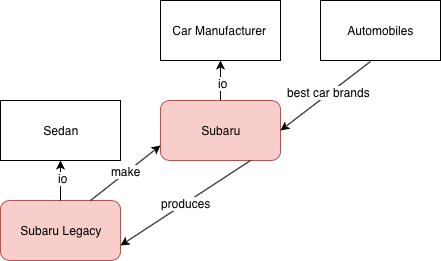
\includegraphics[width=4in]{sample_ontology}
\caption{This sample ontology, with inspiration from an example by Natalya F. Noy, describes entities and relations in the 'automobiles' domain. The ontology serves to provide a "formal explicit description" of classes (outlined in black) along with properties which describe various attributes of the classes (such as how the Subaru Legacy is produced by Subaru). While not displayed in the figure, an ontology also defines property restrictions within the domain (so an instance of the Subaru class cannot produce a car manufacturer). The ontology, along with individual instances of classes (highlighted in red) constitutes a knowledge base \cite{noy2001ontology}. }
\label{fig:sample_ontology}
\end{figure}

 
In reality, few differences between an ontology and a knowledge base exists. Knowledge engineers must traverse a "fine line where the ontology ends and the knowledge base begins" \cite{noy2001ontology}. At the least, an ontology defines categories (or classes) and relationships among objects. One can think of an ontology as a "vocabulary" used to describe a domain \cite[308]{russell2016artificial}. Typically, the classes can be arranged in a hierarchy and the object properties into a separate hierarchy, which are here referred to as semantic hierarchies. When designing an ontology, one must decide the scope and organization of the knowledge, along with the language used to describe a specific domain. Refer to Figure \ref{fig:sample_ontology} for an example. 

RELATIONS  (subclass and subproperty, domain and range restrictions)

\subsubsection{Class and Object Property Inheritance}

 EXPLAIN the terms and they structure knowledge and how inheritance works
 
 

TRANSITION

\begin{figure}[h]
\centering
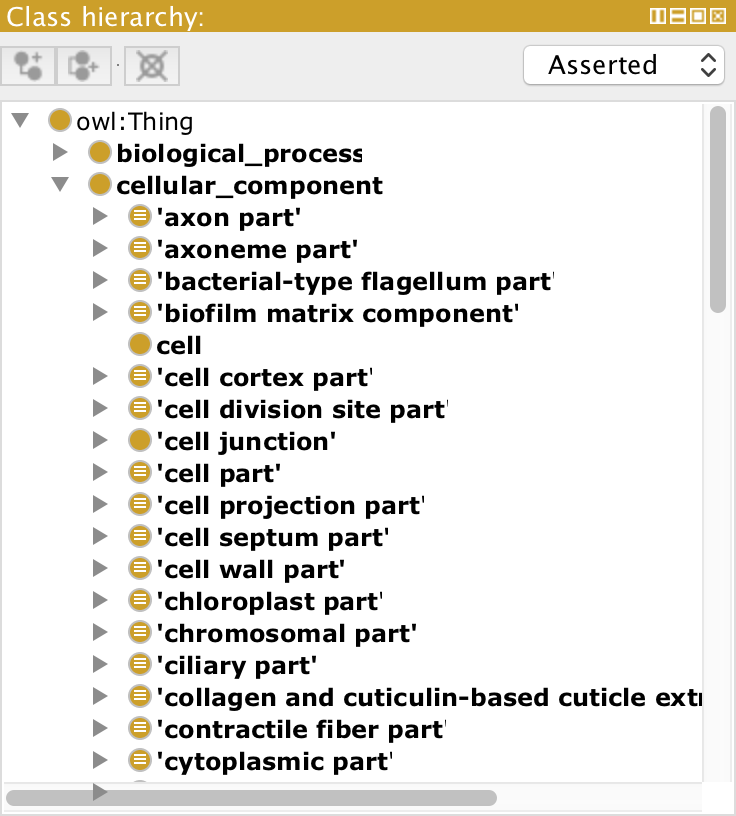
\includegraphics[width=2.5in]{class-hierarchy}
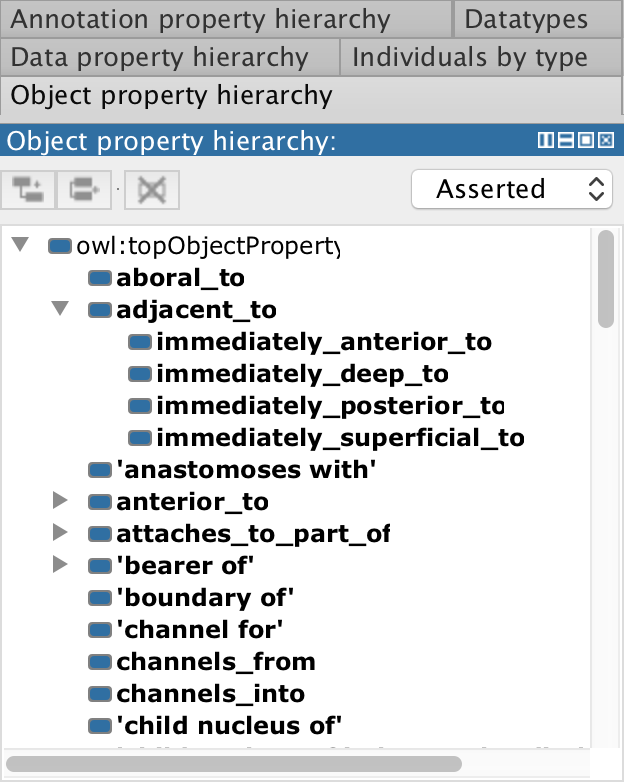
\includegraphics[width=2.5in]{object-property-hierarchy}
\caption{Class hierarchies and object property hierarchies for an ontology can be viewed in Prot{\'e}g{\'e} \cite{gennari2003evolution}. Asserted hierarchies are shown above, and inferred hierarchies are generated by starting the Pellet reasoner.}
\label{fig:class-hierarchy}
\end{figure}

EXAMPLE how the semantic hierarchy may help in a proof (when there are lots of irrelevant axioms).

\subsection{{Theorem Proving}}
Automated theorem proving depends on having an established logic for expressing facts, a method of generating new facts without requiring additional knowledge, and a strategy for searching through all possible new facts one could generate to reach a specific goal (such as proving a conjecture).

\subsubsection{First-order Predicate Logic}

Automatic theorem proving requires a logic defining the syntax of valid statements to run without additional user input. Formal logics like first-order logic, also known as predicate logic and first-order predicate calculus, define a structure for statements which can be used to form logical and mathematical proofs. Consider the following set of asserted facts expressed in first-order predicate logic, commonly referred to as axioms. 

\begin{singlespace}
\[isSedan(Subaru Legacy)\]
\[\forall x \; isSedan(x) \rightarrow hasFourSeats(x)\]
\end{singlespace} 

The first statement asserts the Subaru Legacy is a sedan. The second statement asserts all sedans have four seats. By expressing facts in a formal notation, one makes proofs using such statements mechanical and easily parsed by a computer. Expressing statements in formal logic poses multiple challenges. First, each object and relationship must be explicitly defined.

EXPLAIN FIRST ORDER PREDICATE LOGIC

WHAT is a predicate


\subsubsection{Inference Rules}

One can use axioms to derive facts which logically follow using inference rules. The two previous statements do not directly state the Subaru Legacy has four seats. However, one can derive the statement $hasFourSeats(Subaru Legacy)$ by using the inference rule \textit{modus ponens}, defined below. 
\begin{equation}
\begin{gathered}
A \\
A \rightarrow B \\
\therefore B
\end{gathered}
\end{equation}

One can think of $A$ and $B$ as variables representing statements, and any statement can replace them. An inference rule defines a valid rule for statements. 
\subsubsection{Resolution}

Automated theorem proving requires a set of axioms and a set of rules to generate new facts, but also a strategy to search through the possible applications of the inference rules. Knowledge bases can grow quite large, and generating all possible facts based on a given set of axioms often remains impractical or unfeasible. Resolution exists as historically significant and widely used method for automated theorem proving \cite[51]{ertel2018introduction}. 

\begin{figure}[h]
\centering
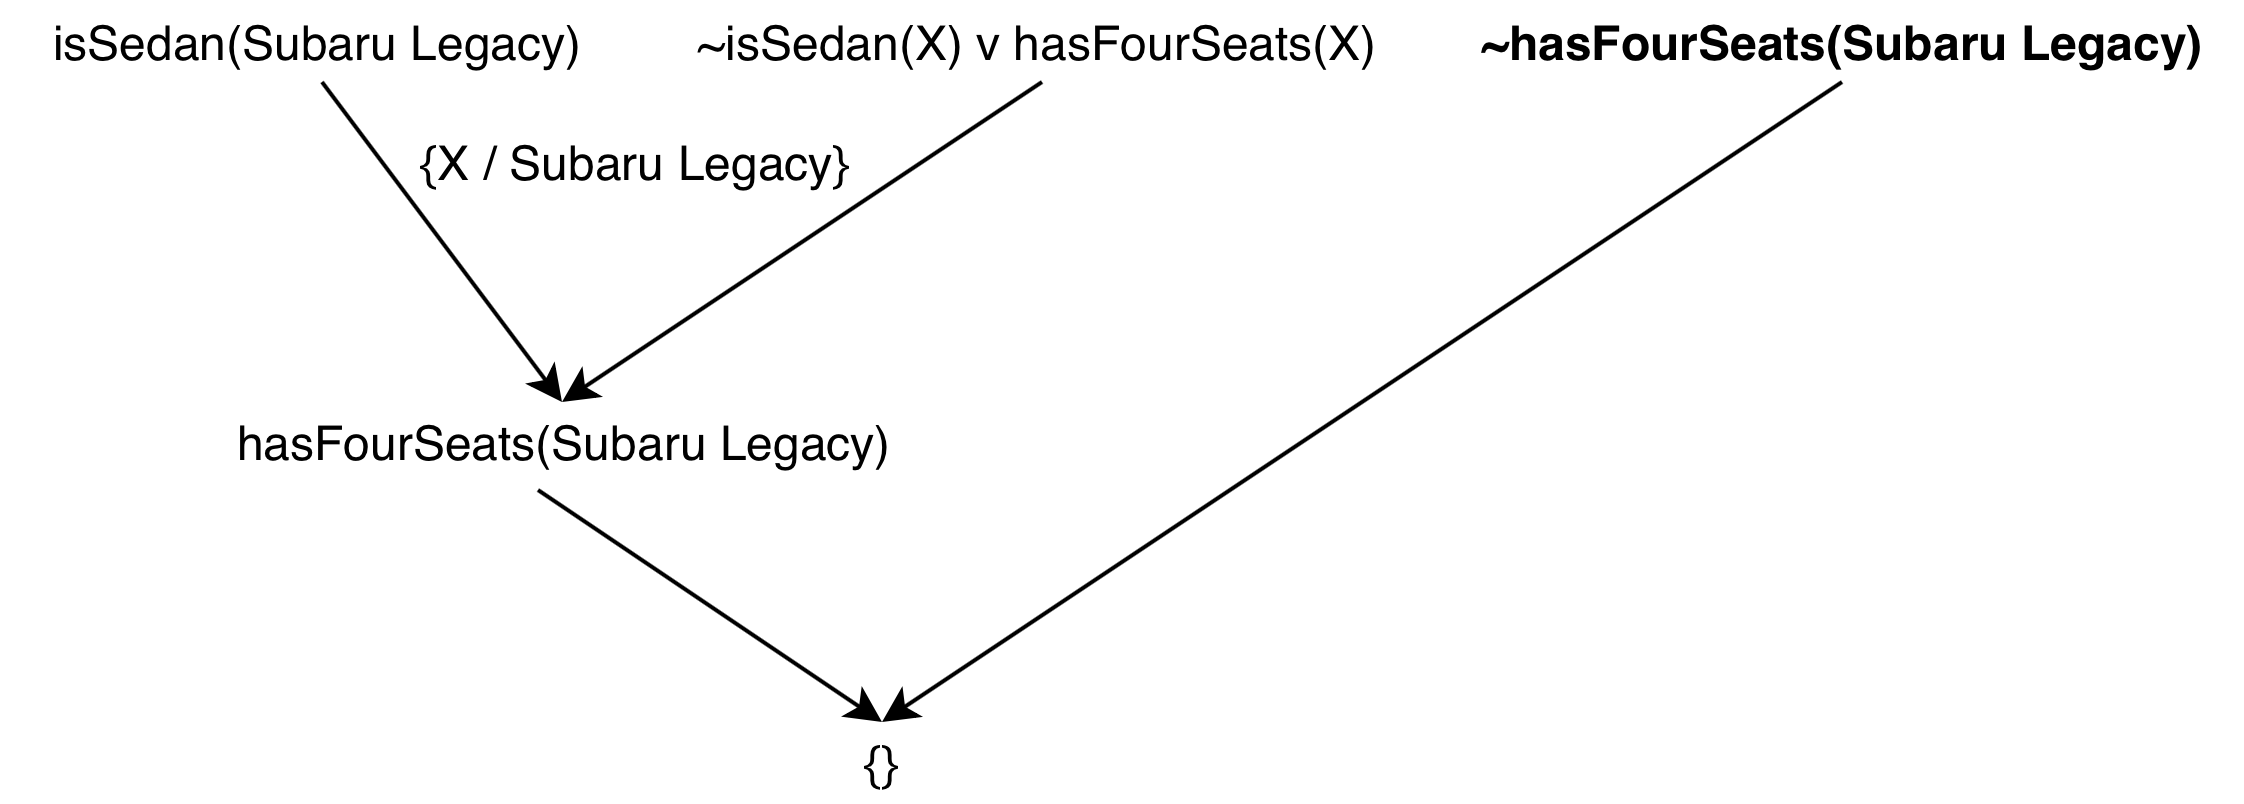
\includegraphics[width=6in]{resolution_tree}
\caption{The figure above displays a resolution tree for the inference rule described in the previous section. The bold statement shows the negated conjecture. The tree also displays $x$ bound to $SubaruLegacy$.}
\label{fig:resolution_tree}
\end{figure}

In order to use resolution as a proof technique, axioms must first be expressed in Conjunctive Normal Form (CNF), also known as clausal form. One may follow a 7-step procedure of converting the set of facts into a conjunction of disjunctions. The process eliminates biconditionals, implications, and quantifiers so the second axiom $\forall x \; isSedan(x) \rightarrow hasFourSeats(x)$ becomes 
$\lnot isSedan(x) \lor hasFourSeats(x)$. One can then resolve the statements by instantiating the variable $x$ with $SubaruLegacy$ in a process called unification, binding the variable. 
\[\frac{isSedan(Subaru Legacy), \lnot isSedan(x) \lor hasFourSeats(x)}{hasFourSeats(Subaru Legacy)}\]
Finally, one can resolve the axiom with the negated conjecture, proving the statement true. 

\begin{figure}[h]
\begin{verbatim}
1 (all x (isSedan(x) -> hasFourSeats(x))) # label(non_clause).  [assumption].
2 hasFourSeats(SubaruLegacy) # label(non_clause) # label(goal).  [goal].
3 -isSedan(x) | hasFourSeats(x).  [clausify(1)].
4 isSedan(SubaruLegacy).  [assumption].
5 hasFourSeats(SubaruLegacy).  [resolve(3,a,4,a)].
6 -hasFourSeats(SubaruLegacy).  [deny(2)].
7 $F.  [resolve(5,a,6,a)].
\end{verbatim}
\caption{Prover9 displays output for the automated proof. }
\label{fig:prover9out}
\end{figure}

As a knowledge base grows, the number of clauses an automated theorem prover can generate greatly increases. Researches have begun to form heuristics to evaluate the relevance of axioms when completing a proof. 

\subsection{Semantic Similarity}
Evaluating the similarity of two entities, or predicates when using a theorem prover, can serve as a heuristic for reducing the number of clauses generated during a proof. Multiple metrics have been developed for evaluating the semantic similarity of terms with different approaches, including: edge-counting measures, feature-based measures, and measures based on Information Content \cite{sanchez2012ontology} \cite{rodriguez1999assessing} \cite{roederer2009divvy}.  Edge-counting metrics for semantic similarity when applied to semantic hierarchies remain the focus of this work. 

Calculating the distance between two entities in an ontology is a a straightforward and intuitive method of calculating the semantic similarity. One can formally define the metric as follows. In an undirected graph $G$ defined as a pair $(V,E)$, where $V$ is a set of vertices, and $E$ is a set of edges between the vertices $E \subseteq {(u,v) | u, v \in V}$, one can define a path $path(a,b)=l_{1,\dots ,}l_k$ as a set of links connecting $a$ and $b$ in a taxonomy and $\lvert path(a,b) \rvert = k$ as the length of the path \cite{sanchez2012ontology}. One can calculate the semantic distance between $a$ and $b$ using equation \ref{rada} \cite{rada1989development}.

\begin{equation}
sim(a,b)=min_{\forall i}\lvert{path_i(a,b)}\rvert
\label{rada}
\end{equation}
By incorporating depth of the taxonomy into the function, improvement has been seen \cite{wu1994verbs}.
\begin{equation}
sim(a,b)=\frac{2 \times N_3}{N_1+N_2+2 \times N_3}
\label{wu}
\end{equation}

\newpage
\vspace*{.05in}
\section{\MakeUppercase{Approach}}
This work aims to evaluate the effectiveness of using a semantic hierarchy generated from an ontology to calculate weights for predicates based on a specific conjecture. In efforts to quantitatively evaluate the effectiveness of the proposed methods, a series of experiments were conducted on multiple ontologies from the COmmon Logic Ontology REpository (COLORE). The objective of COLORE is to serve as a "testbed for ontology evaluation and integration techniques" \cite{gruninger2012specifying}. Code from the project can be found at \url{https://code.google.com/p/colore}. Prot{\'e}g{\'e}, an "open-source ontology editor and framework for building intelligent systems" was used to generate the semantic hierarchies. The ontologies had to first be converted into a format Prot{\'e}g{\'e} can read. Then, Prot{\'e}g{\'e}, along with a semantic reasoner, were used to generate both a class hierarchy and an object property hierarchy for each ontology. The semantic hierarchies were then used to calculate the assigned weights for each predicate when executing proofs. Finally, tests were run using Prover9 to compare the default weights to the calculated weights. The effectiveness of the process was evaluated by comparing the number of clauses generated by Prover9 for each proof. 

\begin{figure}[h]
\centering
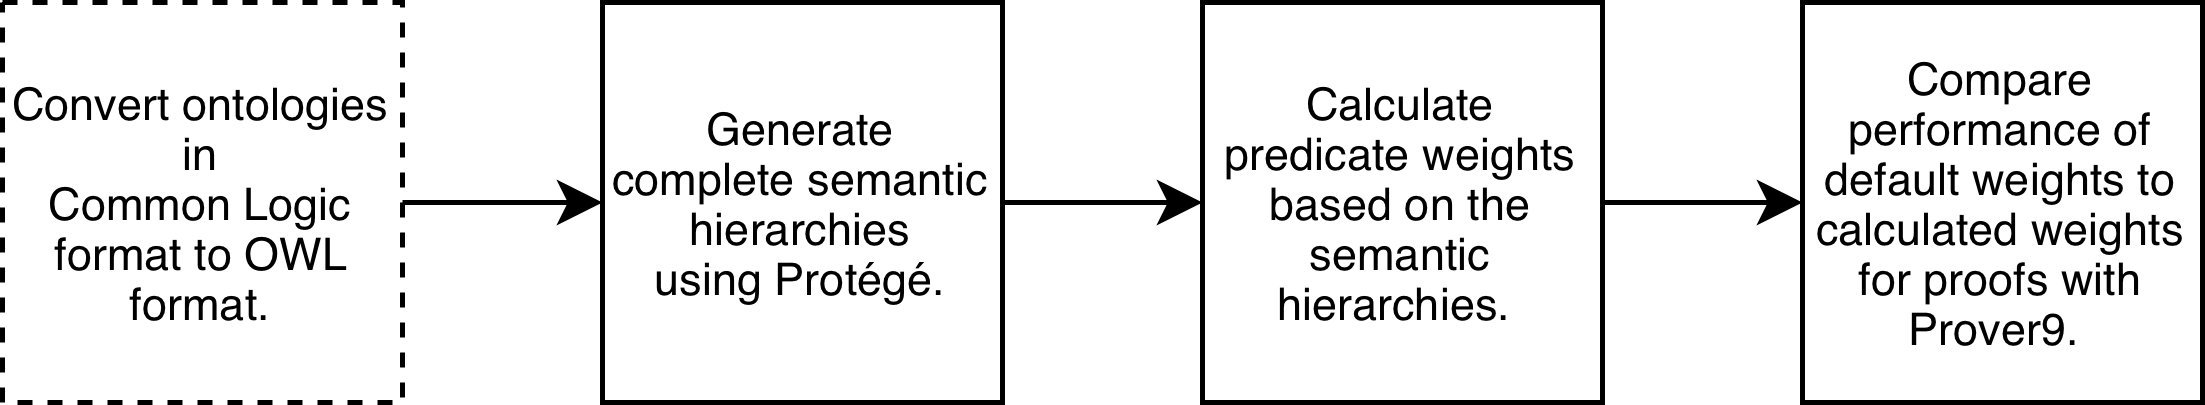
\includegraphics[width=6in]{flowchart}
\caption{The figure above illustrates my process of conducting experiments. The first step, converting the ontologies into a formate readable Prot{\'e}g{\'e}, lives outside of the scope of my research.}
\label{fig:flowchart}
\end{figure}

\subsection{Converting Ontologies}
Dr. Michael Gr\"{u}inger specified ontologies contained in COLORE using Common Logic. One must convert the ontologies from the Common Logic Interchange Format (CLIF) to the Web Ontology Language (OWL) in order to view the ontology in Prot{\'e}g{\'e} and generate the semantic hierarchies. Robert Powell has written a utility which executes the conversion and has generated the files necessary to conduct this research. 

COLORE contains the knowledge base for each ontology. Additionally, one finds the conjectures used to test each ontology at \url{https://github.com/gruninger/colore/tree/master/ontologies}. Not all ontologies in COLORE have conjectures, which limits the scope of my experiments to the sufficiently large ontologies with multiple defined conjectures to test. 

\subsection{Generating a Complete Heirarchy}
After opening an ontology defined using the OWL format in Prot{\'e}g{\'e}, one can generate both a class hierarchy and an object property hierarchy for including both asserted relationships and inferred relationships. Prot{\'e}g{\'e} generates a view of inferred semantic hierarchies (shown in Figure \ref{fig:class-hierarchy}) using a semantic reasoner called Pellet. The reasoner parses the axioms for inferred logical consequences (i.e. relationships between classes) not explicitly defined. The reasoner generates more complete and accurate semantic hierarchies. 

Given an ontology and a conjecture, one can generate weights for classes and properties to reduce the number of clauses generated in a proof. Functions are evaluated by their influence on the number of clauses generated with a proof. 

After a hierarchy has been generated, weights can be assigned to each class and subproperty. The same weighting function is applied to both the classes and sub-properties. 

The weighting functions are currently applied by hand to the ontologies, with the beginnings of an automated program underway. 



\subsection{Understanding Default Weights}
Prover9 assigns weights to predicates automatically unless the user explicitly defines them. An understanding of the process helps one to develop new weights for the predicates. Rules for weighting axioms in terms of relevance when attempting to prove a specific conjecture are as follows \cite{mccune2005prover9}: 

\begin{singlespace}
\centering
\begin{itemize}
    \item The default weight of a constant or variable is 1.
    \item The default weight of a term or atomic formula is one more than the sum of the weights of its arguments.
    \item The default weight of a literal is the weight of its atomic formula.
    \item The default weight of a clause is the sum of the weights of its literals.
\end{itemize}
\end{singlespace}

One can assign weights to predicates explicitly, 

\subsection{Calculating Weights}
Two explicit weighting functions inspired by related works in calculating semantic similarity, were formed and tested. The weights for each conjecture were then calculated by hand and entered into a spreadsheet. A python script was used to generate the input files used by Prover9 from the spreadsheet for each conjecture. The calculated weights were then entered into Prover9 as additional input along with the axioms and the conjecture. 

\newpage
\vspace*{.05in}
\section{\MakeUppercase{Experiments}}

\subsection{{Setup}}

Experiments were conducted using Prover9, an "automated theorem prover for first-order and equational logic" written by William McCune \cite{mccune2005prover9}. Many tests were conducted using a version of the program which supports a Graphical User Interface (GUI), but a command line version, useful for running automated tests, exists. 
Git was used for version control and a repository containing source code for tests can be found at \url{https://github.com/stanleysmall/thesis}.
\begin{figure}[h]
\centering
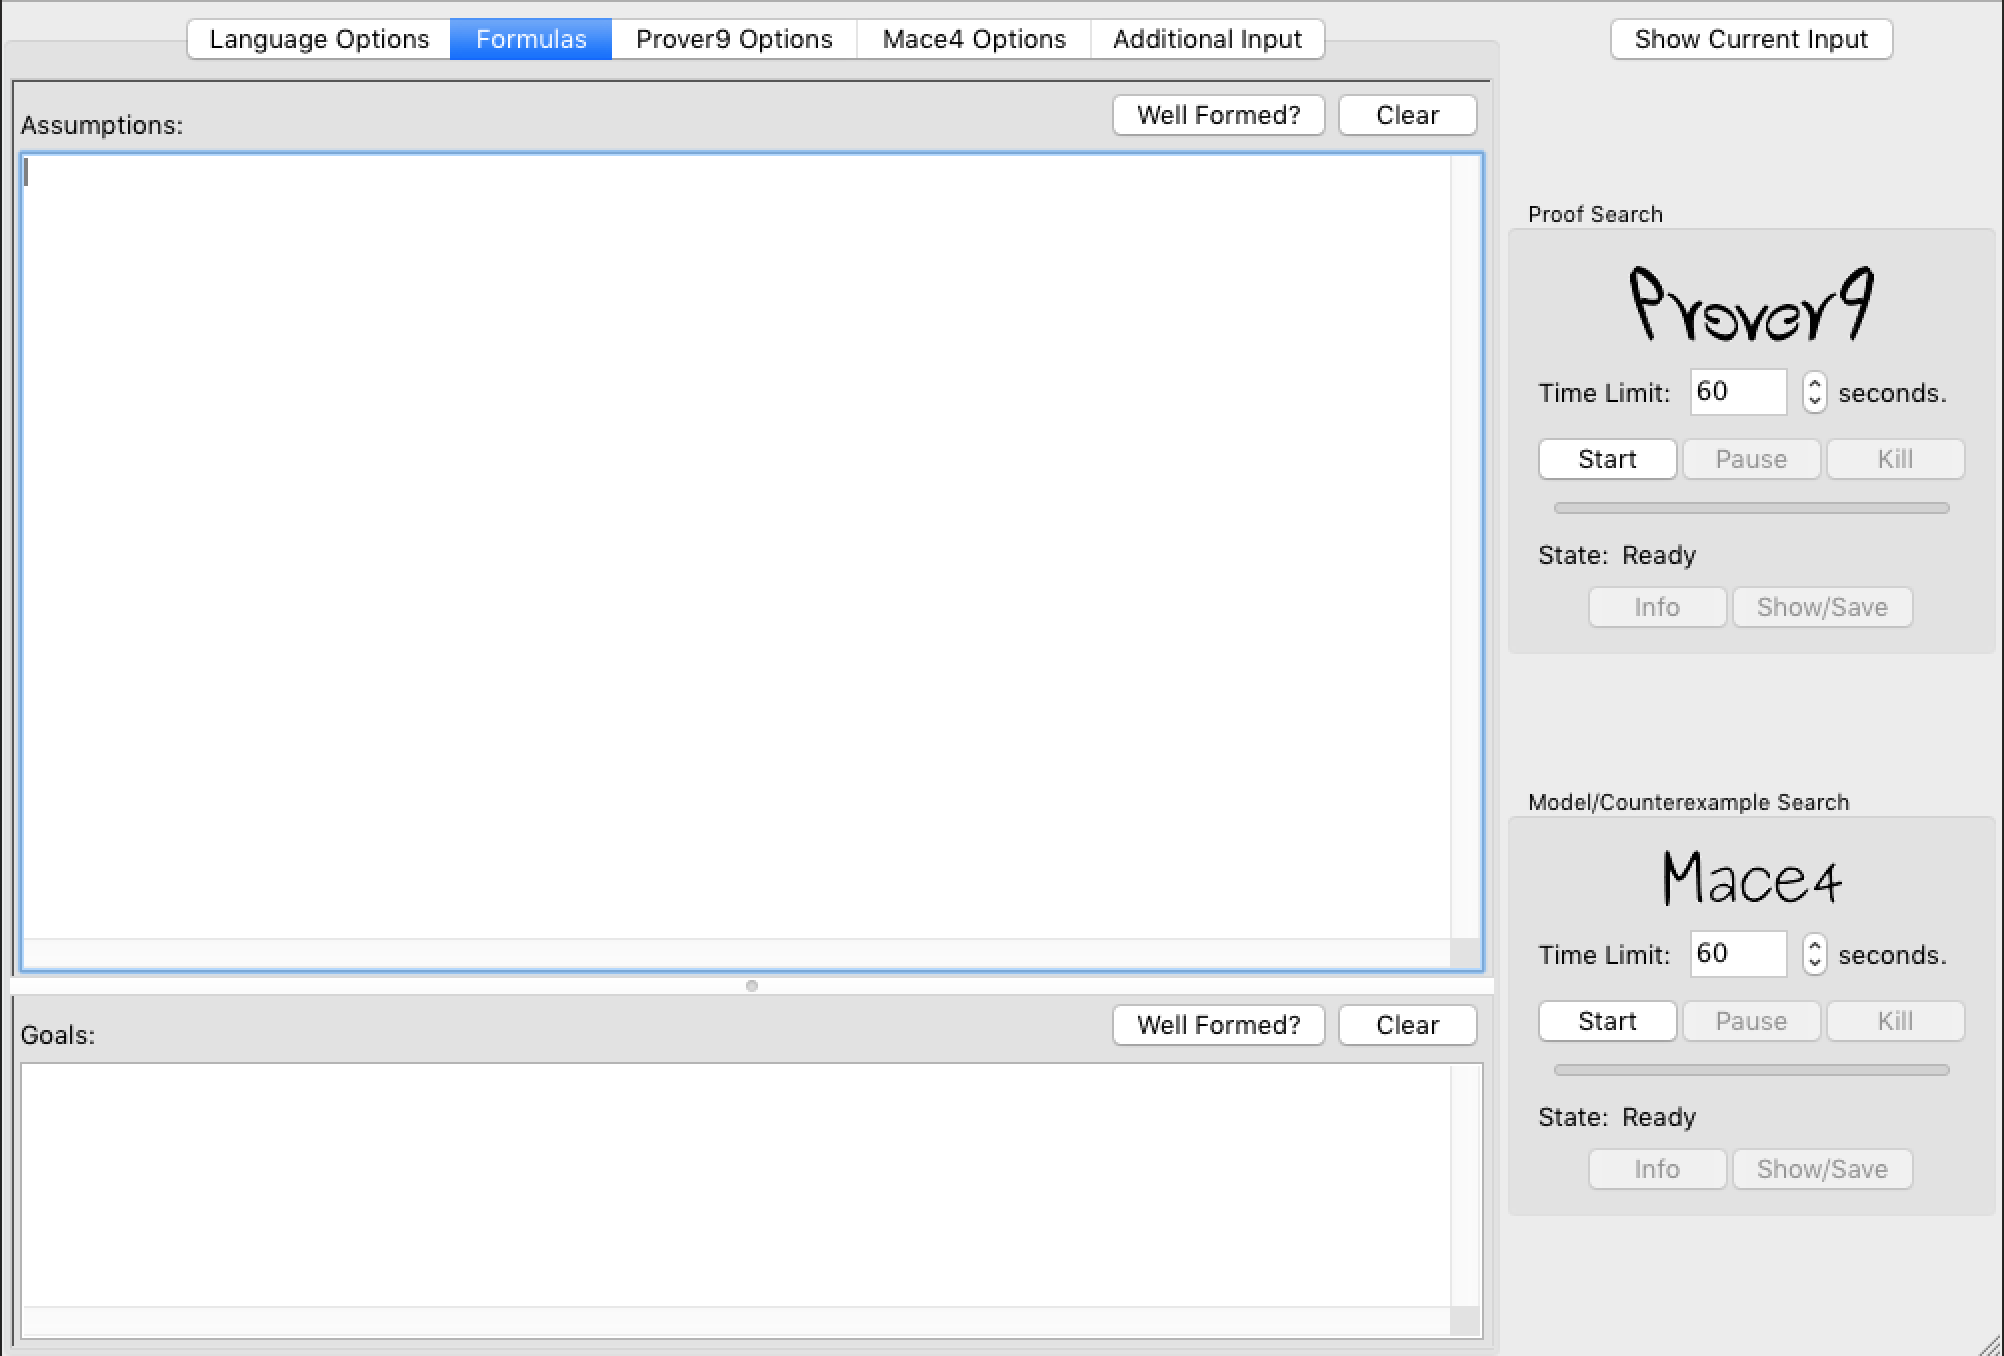
\includegraphics[width=6in]{prover9}
\caption{The GUI for Prover9 on macOS is shown above. One enters axioms into the top text field and conjectures into the bottom text field. Predicate weights are entered in the 'Additional Input' tab in the navigation bar. Users can start the proof by pressing the 'Start' button below the Prover9 logo after specifying a time limit. After the proof has completed, users can view the number of clauses generated by the proof by pressing the 'Info' button below the 'Start' button \cite{mccune2005prover9}.}
\label{fig:prover9}
\end{figure}

\subsection{Weighting Functions}
Two weighting functions were defined for testing. 

\subsection{{Results}}
\subsubsection{multidim\_space\_voids}
\begin{table}[h]
\centering
\csvautotabular{tests/multidim_space_voids/results.csv}
\caption{Results for the multidim\_space\_voids Ontology}
\end{table}

\newpage
\vspace*{.05in}
\section{\MakeUppercase{Conclusions}}

In many cases, the algorithm increases the number of clauses generated for each test, but does not do so to the point where the tests are unusable. For some very specific ontologies, the number of clauses generated decreases. This can be attributed to, in part, by the small number of ontologies available for testing, along with the specific pattern and hierarchy of each ontology. 

Many opportunities for further research include fully automating the search procedure, working with a larger number of ontologies to ensure the weighting functions actually do as they say, developing a new approach towards automatically weighting the predicates. 
\newpage
\addcontentsline{toc}{section}{\MakeUppercase{References}}
\vspace*{.05in}
\printbibliography

\newpage
\appendix
\section{\MakeUppercase{Tests}}
\begin{singlespace}
\csvautolongtable[
      table head=\caption{multidim space voids weights}\label{tab:some}\\\hline
               \csvlinetotablerow\\\hline
               \endfirsthead\hline
               \csvlinetotablerow\\\hline
               \endhead\hline
               \endfoot,
               respect all
               ]{tests/multidim_space_voids/weights.csv}
\end{singlespace}


\newpage
\addcontentsline{toc}{section}{\MakeUppercase{Author's Biography}}
\vspace*{.05in}
\section*{\MakeUppercase{Author's Biography}}
Stanley C. Small grew up in Hampden, Maine with his mother Diane and his father Scott. He attended the University of Maine and received a Bachelor of Science degree in Computer Science in May of 2019. 


\end{document}
